\documentclass{standalone}
\usepackage{tikz}
\usetikzlibrary{patterns, positioning}


\begin{document}
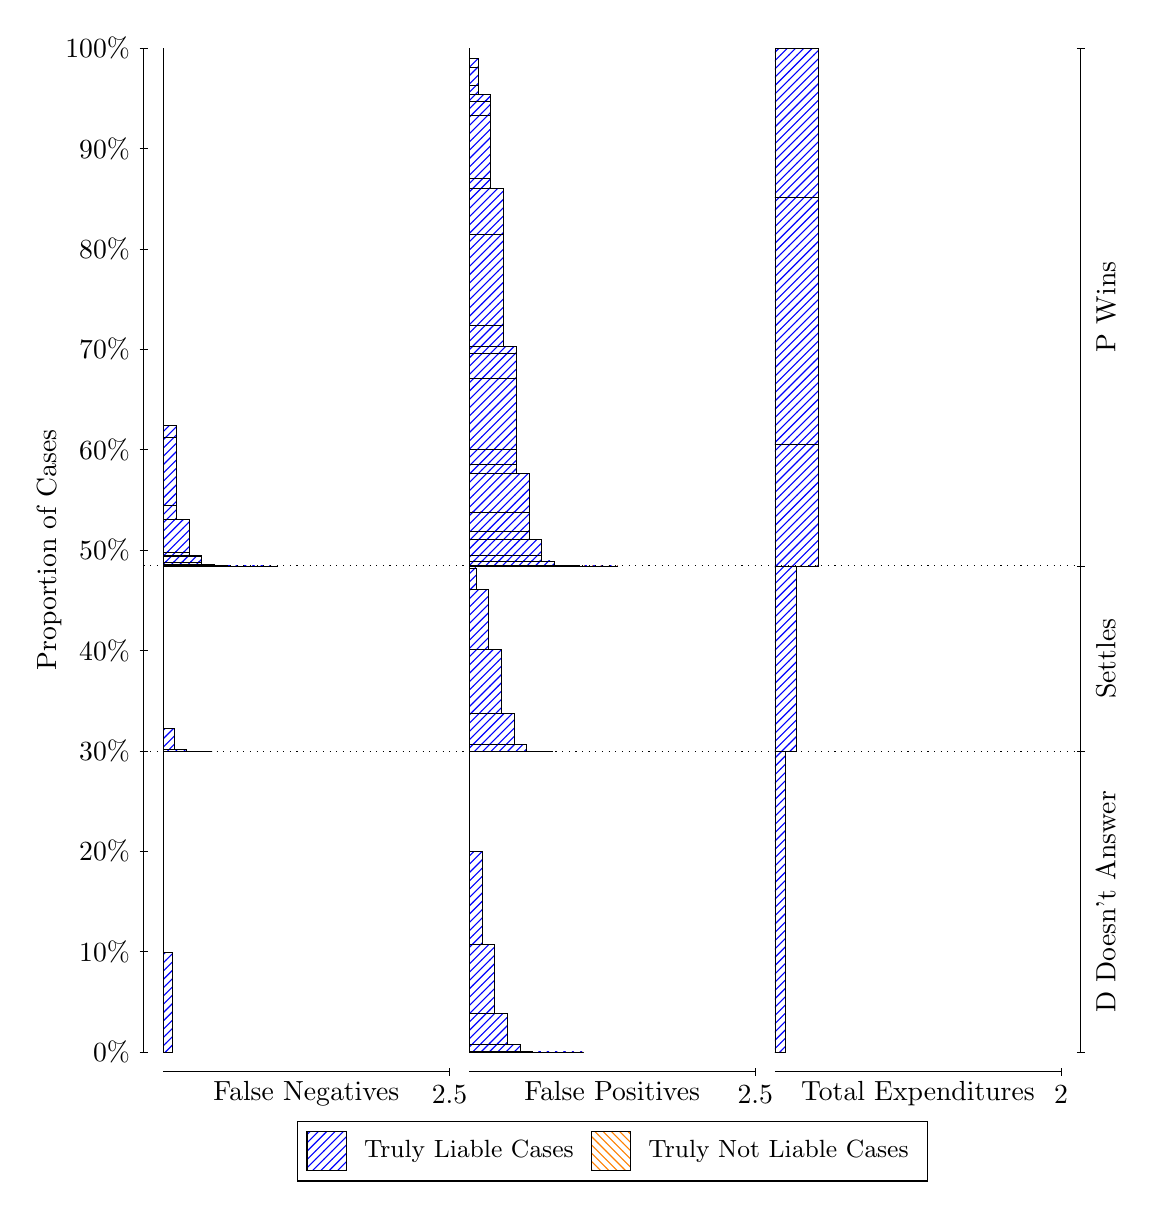
\begin{tikzpicture}
\draw[black, very thin] (1.5,1.75) -- (1.5,14.5);
\node[rotate=90, text=black, anchor=center] at (0.3, 8.125) {Proportion of Cases};
\draw[black, very thin] (1.45,1.75) -- (1.55,1.75);
\node[text=black, anchor=east] at (1.45, 1.75) {0\%};
\draw[black, very thin] (1.45,3.025) -- (1.55,3.025);
\node[text=black, anchor=east] at (1.45, 3.025) {10\%};
\draw[black, very thin] (1.45,4.3) -- (1.55,4.3);
\node[text=black, anchor=east] at (1.45, 4.3) {20\%};
\draw[black, very thin] (1.45,5.575) -- (1.55,5.575);
\node[text=black, anchor=east] at (1.45, 5.575) {30\%};
\draw[black, very thin] (1.45,6.85) -- (1.55,6.85);
\node[text=black, anchor=east] at (1.45, 6.85) {40\%};
\draw[black, very thin] (1.45,8.125) -- (1.55,8.125);
\node[text=black, anchor=east] at (1.45, 8.125) {50\%};
\draw[black, very thin] (1.45,9.4) -- (1.55,9.4);
\node[text=black, anchor=east] at (1.45, 9.4) {60\%};
\draw[black, very thin] (1.45,10.675) -- (1.55,10.675);
\node[text=black, anchor=east] at (1.45, 10.675) {70\%};
\draw[black, very thin] (1.45,11.95) -- (1.55,11.95);
\node[text=black, anchor=east] at (1.45, 11.95) {80\%};
\draw[black, very thin] (1.45,13.225) -- (1.55,13.225);
\node[text=black, anchor=east] at (1.45, 13.225) {90\%};
\draw[black, very thin] (1.45,14.5) -- (1.55,14.5);
\node[text=black, anchor=east] at (1.45, 14.5) {100\%};

\draw[black, very thin] (13.4,1.75) -- (13.4,14.5);
\draw[black, very thin] (13.35,1.75) -- (13.45,1.75);
\node[anchor=west] at (13.35, 1.75) {};
\draw[black, very thin] (13.35,5.5631) -- (13.45,5.5631);
\node[anchor=west] at (13.35, 5.5631) {};
\draw[black, very thin] (13.35,7.9244) -- (13.45,7.9244);
\node[anchor=west] at (13.35, 7.9244) {};
\draw[black, very thin] (13.35,14.5) -- (13.45,14.5);
\node[anchor=west] at (13.35, 14.5) {};

\draw[black, very thin, pattern color=blue, pattern=north east lines] (1.75,1.75) rectangle (1.859,3.0136);
\draw[black, very thin, pattern color=orange, pattern=north west lines] (1.75,3.0136) rectangle (1.75,3.0136);
\draw[black, very thin, pattern color=blue, pattern=north east lines] (1.75,3.0136) rectangle (1.75,5.5631);
\draw[black, very thin, pattern color=blue, pattern=north east lines] (1.75,5.5631) rectangle (2.3677,5.5631);
\draw[black, very thin, pattern color=blue, pattern=north east lines] (1.75,5.5631) rectangle (2.2062,5.5637);
\draw[black, very thin, pattern color=blue, pattern=north east lines] (1.75,5.5637) rectangle (2.0447,5.5903);
\draw[black, very thin, pattern color=blue, pattern=north east lines] (1.75,5.5903) rectangle (1.8832,5.8599);
\draw[black, very thin, pattern color=orange, pattern=north west lines] (1.75,5.8599) rectangle (1.75,5.8599);
\draw[black, very thin, pattern color=blue, pattern=north east lines] (1.75,5.8599) rectangle (1.75,7.9244);
\draw[black, very thin, pattern color=blue, pattern=north east lines] (1.75,7.9244) rectangle (3.2033,7.9244);
\draw[black, very thin, pattern color=blue, pattern=north east lines] (1.75,7.9244) rectangle (3.0419,7.9244);
\draw[black, very thin, pattern color=blue, pattern=north east lines] (1.75,7.9244) rectangle (2.8804,7.9244);
\draw[black, very thin, pattern color=blue, pattern=north east lines] (1.75,7.9244) rectangle (2.8804,7.9244);
\draw[black, very thin, pattern color=blue, pattern=north east lines] (1.75,7.9244) rectangle (2.7189,7.9245);
\draw[black, very thin, pattern color=blue, pattern=north east lines] (1.75,7.9245) rectangle (2.7189,7.9245);
\draw[black, very thin, pattern color=blue, pattern=north east lines] (1.75,7.9245) rectangle (2.5574,7.9265);
\draw[black, very thin, pattern color=blue, pattern=north east lines] (1.75,7.9265) rectangle (2.3959,7.9334);
\draw[black, very thin, pattern color=blue, pattern=north east lines] (1.75,7.9334) rectangle (2.3959,7.9435);
\draw[black, very thin, pattern color=blue, pattern=north east lines] (1.75,7.9435) rectangle (2.2344,7.9751);
\draw[black, very thin, pattern color=blue, pattern=north east lines] (1.75,7.9751) rectangle (2.2344,8.0497);
\draw[black, very thin, pattern color=blue, pattern=north east lines] (1.75,8.0497) rectangle (2.2344,8.0538);
\draw[black, very thin, pattern color=blue, pattern=north east lines] (1.75,8.0538) rectangle (2.073,8.1011);
\draw[black, very thin, pattern color=blue, pattern=north east lines] (1.75,8.1011) rectangle (2.073,8.5141);
\draw[black, very thin, pattern color=blue, pattern=north east lines] (1.75,8.5141) rectangle (1.9115,8.6896);
\draw[black, very thin, pattern color=blue, pattern=north east lines] (1.75,8.6896) rectangle (1.9115,9.5537);
\draw[black, very thin, pattern color=blue, pattern=north east lines] (1.75,9.5537) rectangle (1.9115,9.7068);
\draw[black, very thin, pattern color=orange, pattern=north west lines] (1.75,9.7068) rectangle (1.75,9.7068);
\draw[black, very thin, pattern color=blue, pattern=north east lines] (1.75,9.7068) rectangle (1.75,14.5);
\draw[black, very thin, pattern color=orange, pattern=north west lines] (5.6333,1.75) rectangle (7.0867,1.75);
\draw[black, very thin, pattern color=blue, pattern=north east lines] (5.6333,1.75) rectangle (7.0867,1.75);
\draw[black, very thin, pattern color=blue, pattern=north east lines] (5.6333,1.75) rectangle (6.9252,1.75);
\draw[black, very thin, pattern color=blue, pattern=north east lines] (5.6333,1.75) rectangle (6.7637,1.75);
\draw[black, very thin, pattern color=blue, pattern=north east lines] (5.6333,1.75) rectangle (6.6022,1.7503);
\draw[black, very thin, pattern color=blue, pattern=north east lines] (5.6333,1.7503) rectangle (6.4407,1.7582);
\draw[black, very thin, pattern color=blue, pattern=north east lines] (5.6333,1.7582) rectangle (6.2793,1.8434);
\draw[black, very thin, pattern color=blue, pattern=north east lines] (5.6333,1.8434) rectangle (6.1178,2.2366);
\draw[black, very thin, pattern color=blue, pattern=north east lines] (5.6333,2.2366) rectangle (5.9563,3.1157);
\draw[black, very thin, pattern color=blue, pattern=north east lines] (5.6333,3.1157) rectangle (5.7948,4.2995);
\draw[black, very thin, pattern color=blue, pattern=north east lines] (5.6333,4.2995) rectangle (5.6333,5.5631);
\draw[black, very thin, pattern color=orange, pattern=north west lines] (5.6333,5.5631) rectangle (6.687,5.5631);
\draw[black, very thin, pattern color=blue, pattern=north east lines] (5.6333,5.5631) rectangle (6.687,5.5635);
\draw[black, very thin, pattern color=blue, pattern=north east lines] (5.6333,5.5635) rectangle (6.5255,5.572);
\draw[black, very thin, pattern color=blue, pattern=north east lines] (5.6333,5.572) rectangle (6.364,5.6577);
\draw[black, very thin, pattern color=blue, pattern=north east lines] (5.6333,5.6577) rectangle (6.2026,6.0484);
\draw[black, very thin, pattern color=blue, pattern=north east lines] (5.6333,6.0484) rectangle (6.0411,6.8637);
\draw[black, very thin, pattern color=blue, pattern=north east lines] (5.6333,6.8637) rectangle (5.8796,7.6275);
\draw[black, very thin, pattern color=blue, pattern=north east lines] (5.6333,7.6275) rectangle (5.7181,7.8972);
\draw[black, very thin, pattern color=blue, pattern=north east lines] (5.6333,7.8972) rectangle (5.6333,7.9244);
\draw[black, very thin, pattern color=orange, pattern=north west lines] (5.6333,7.9244) rectangle (7.5227,7.9244);
\draw[black, very thin, pattern color=blue, pattern=north east lines] (5.6333,7.9244) rectangle (7.5227,7.9244);
\draw[black, very thin, pattern color=orange, pattern=north west lines] (5.6333,7.9244) rectangle (7.3612,7.9244);
\draw[black, very thin, pattern color=blue, pattern=north east lines] (5.6333,7.9244) rectangle (7.3612,7.9244);
\draw[black, very thin, pattern color=blue, pattern=north east lines] (5.6333,7.9244) rectangle (7.1997,7.9244);
\draw[black, very thin, pattern color=orange, pattern=north west lines] (5.6333,7.9244) rectangle (7.1997,7.9244);
\draw[black, very thin, pattern color=blue, pattern=north east lines] (5.6333,7.9244) rectangle (7.1997,7.9245);
\draw[black, very thin, pattern color=blue, pattern=north east lines] (5.6333,7.9245) rectangle (7.0382,7.9246);
\draw[black, very thin, pattern color=blue, pattern=north east lines] (5.6333,7.9246) rectangle (7.0382,7.9247);
\draw[black, very thin, pattern color=orange, pattern=north west lines] (5.6333,7.9247) rectangle (7.0382,7.9247);
\draw[black, very thin, pattern color=blue, pattern=north east lines] (5.6333,7.9247) rectangle (7.0382,7.9251);
\draw[black, very thin, pattern color=orange, pattern=north west lines] (5.6333,7.9251) rectangle (6.8767,7.9251);
\draw[black, very thin, pattern color=blue, pattern=north east lines] (5.6333,7.9251) rectangle (6.8767,7.9292);
\draw[black, very thin, pattern color=blue, pattern=north east lines] (5.6333,7.9292) rectangle (6.8767,7.9308);
\draw[black, very thin, pattern color=blue, pattern=north east lines] (5.6333,7.9308) rectangle (6.8767,7.9326);
\draw[black, very thin, pattern color=orange, pattern=north west lines] (5.6333,7.9326) rectangle (6.7153,7.9326);
\draw[black, very thin, pattern color=blue, pattern=north east lines] (5.6333,7.9326) rectangle (6.7153,7.9775);
\draw[black, very thin, pattern color=blue, pattern=north east lines] (5.6333,7.9775) rectangle (6.7153,7.988);
\draw[black, very thin, pattern color=blue, pattern=north east lines] (5.6333,7.988) rectangle (6.5538,8.0589);
\draw[black, very thin, pattern color=orange, pattern=north west lines] (5.6333,8.0589) rectangle (6.5538,8.0589);
\draw[black, very thin, pattern color=blue, pattern=north east lines] (5.6333,8.0589) rectangle (6.5538,8.2602);
\draw[black, very thin, pattern color=blue, pattern=north east lines] (5.6333,8.2602) rectangle (6.3923,8.3591);
\draw[black, very thin, pattern color=blue, pattern=north east lines] (5.6333,8.3591) rectangle (6.3923,8.6091);
\draw[black, very thin, pattern color=orange, pattern=north west lines] (5.6333,8.6091) rectangle (6.3923,8.6091);
\draw[black, very thin, pattern color=blue, pattern=north east lines] (5.6333,8.6091) rectangle (6.3923,9.0976);
\draw[black, very thin, pattern color=blue, pattern=north east lines] (5.6333,9.0976) rectangle (6.2308,9.2156);
\draw[black, very thin, pattern color=blue, pattern=north east lines] (5.6333,9.2156) rectangle (6.2308,9.4038);
\draw[black, very thin, pattern color=orange, pattern=north west lines] (5.6333,9.4038) rectangle (6.2308,9.4038);
\draw[black, very thin, pattern color=blue, pattern=north east lines] (5.6333,9.4038) rectangle (6.2308,10.305);
\draw[black, very thin, pattern color=blue, pattern=north east lines] (5.6333,10.305) rectangle (6.2308,10.623);
\draw[black, very thin, pattern color=blue, pattern=north east lines] (5.6333,10.623) rectangle (6.2308,10.712);
\draw[black, very thin, pattern color=blue, pattern=north east lines] (5.6333,10.712) rectangle (6.0693,10.975);
\draw[black, very thin, pattern color=orange, pattern=north west lines] (5.6333,10.975) rectangle (6.0693,10.975);
\draw[black, very thin, pattern color=blue, pattern=north east lines] (5.6333,10.975) rectangle (6.0693,12.129);
\draw[black, very thin, pattern color=blue, pattern=north east lines] (5.6333,12.129) rectangle (6.0693,12.718);
\draw[black, very thin, pattern color=blue, pattern=north east lines] (5.6333,12.718) rectangle (5.9079,12.848);
\draw[black, very thin, pattern color=blue, pattern=north east lines] (5.6333,12.848) rectangle (5.9079,13.64);
\draw[black, very thin, pattern color=blue, pattern=north east lines] (5.6333,13.64) rectangle (5.9079,13.829);
\draw[black, very thin, pattern color=blue, pattern=north east lines] (5.6333,13.829) rectangle (5.9079,13.91);
\draw[black, very thin, pattern color=blue, pattern=north east lines] (5.6333,13.91) rectangle (5.7464,14.022);
\draw[black, very thin, pattern color=blue, pattern=north east lines] (5.6333,14.022) rectangle (5.7464,14.259);
\draw[black, very thin, pattern color=blue, pattern=north east lines] (5.6333,14.259) rectangle (5.7464,14.371);
\draw[black, very thin, pattern color=blue, pattern=north east lines] (5.6333,14.371) rectangle (5.6333,14.5);
\draw[black, very thin, pattern color=orange, pattern=north west lines] (9.5167,1.75) rectangle (9.6529,1.75);
\draw[black, very thin, pattern color=blue, pattern=north east lines] (9.5167,1.75) rectangle (9.6529,5.5631);
\draw[black, very thin, pattern color=orange, pattern=north west lines] (9.5167,5.5631) rectangle (9.7892,5.5631);
\draw[black, very thin, pattern color=blue, pattern=north east lines] (9.5167,5.5631) rectangle (9.7892,7.9244);
\draw[black, very thin, pattern color=orange, pattern=north west lines] (9.5167,7.9244) rectangle (10.062,7.9244);
\draw[black, very thin, pattern color=blue, pattern=north east lines] (9.5167,7.9244) rectangle (10.062,9.4653);
\draw[black, very thin, pattern color=orange, pattern=north west lines] (9.5167,9.4653) rectangle (10.062,9.4653);
\draw[black, very thin, pattern color=blue, pattern=north east lines] (9.5167,9.4653) rectangle (10.062,12.6);
\draw[black, very thin, pattern color=orange, pattern=north west lines] (9.5167,12.6) rectangle (10.062,12.6);
\draw[black, very thin, pattern color=blue, pattern=north east lines] (9.5167,12.6) rectangle (10.062,14.5);
\draw[black, dotted] (1.5,5.5631) -- (13.4,5.5631);
\draw[black, dotted] (1.5,7.9244) -- (13.4,7.9244);
\draw[black, very thin] (1.75,1.5) -- (5.3833,1.5);
\node[text=black, anchor=north] at (3.5667, 1.5) {False Negatives};
\draw[black, very thin] (5.3833,1.45) -- (5.3833,1.55);
\node[text=black, anchor=north] at (5.3833, 1.45) {2.5};

\draw[black, very thin] (5.6333,1.5) -- (9.2667,1.5);
\node[text=black, anchor=north] at (7.45, 1.5) {False Positives};
\draw[black, very thin] (9.2667,1.45) -- (9.2667,1.55);
\node[text=black, anchor=north] at (9.2667, 1.45) {2.5};

\draw[black, very thin] (9.5167,1.5) -- (13.15,1.5);
\node[text=black, anchor=north] at (11.333, 1.5) {Total Expenditures};
\draw[black, very thin] (13.15,1.45) -- (13.15,1.55);
\node[text=black, anchor=north] at (13.15, 1.45) {2};

\node[text=black, centered, rotate=90] at (13.72, 3.6565) {D Doesn't Answer};
\node[text=black, centered, rotate=90] at (13.72, 6.7437) {Settles};
\node[text=black, centered, rotate=90] at (13.72, 11.212) {P Wins};

\draw (7.449999999999999,1.5) node[draw=none] (baseCoordinate) {};
\begin{scope}[align=center]
        \matrix[scale=0.5, draw=black, below=0.5cm of baseCoordinate, nodes={draw}, column sep=0.1cm]{
            \node[rectangle, draw, minimum width=0.5cm, minimum height=0.5cm, pattern color=blue, pattern=north east lines] {}; &
            \node[draw=none, font=\small, text=black] (B) {Truly Liable Cases}; &
            \node[rectangle, draw, minimum width=0.5cm, minimum height=0.5cm, pattern color=orange, pattern=north west lines] {}; &
            \node[draw=none, font=\small, text=black] (B) {Truly Not Liable Cases}; \\
            };
\end{scope}

\end{tikzpicture}
\end{document}